% Options for packages loaded elsewhere
\PassOptionsToPackage{unicode}{hyperref}
\PassOptionsToPackage{hyphens}{url}
%
\documentclass[
]{article}
\usepackage{lmodern}
\usepackage{amssymb,amsmath}
\usepackage{ifxetex,ifluatex}
\ifnum 0\ifxetex 1\fi\ifluatex 1\fi=0 % if pdftex
  \usepackage[T1]{fontenc}
  \usepackage[utf8]{inputenc}
  \usepackage{textcomp} % provide euro and other symbols
\else % if luatex or xetex
  \usepackage{unicode-math}
  \defaultfontfeatures{Scale=MatchLowercase}
  \defaultfontfeatures[\rmfamily]{Ligatures=TeX,Scale=1}
\fi
% Use upquote if available, for straight quotes in verbatim environments
\IfFileExists{upquote.sty}{\usepackage{upquote}}{}
\IfFileExists{microtype.sty}{% use microtype if available
  \usepackage[]{microtype}
  \UseMicrotypeSet[protrusion]{basicmath} % disable protrusion for tt fonts
}{}
\makeatletter
\@ifundefined{KOMAClassName}{% if non-KOMA class
  \IfFileExists{parskip.sty}{%
    \usepackage{parskip}
  }{% else
    \setlength{\parindent}{0pt}
    \setlength{\parskip}{6pt plus 2pt minus 1pt}}
}{% if KOMA class
  \KOMAoptions{parskip=half}}
\makeatother
\usepackage{xcolor}
\IfFileExists{xurl.sty}{\usepackage{xurl}}{} % add URL line breaks if available
\IfFileExists{bookmark.sty}{\usepackage{bookmark}}{\usepackage{hyperref}}
\hypersetup{
  pdftitle={Use the MRP model to predict the overall popular vote in the Canadian Federal Election in 2019},
  pdfauthor={Xiaoxi Bai(1004144749)},
  hidelinks,
  pdfcreator={LaTeX via pandoc}}
\urlstyle{same} % disable monospaced font for URLs
\usepackage[margin=1in]{geometry}
\usepackage{graphicx,grffile}
\makeatletter
\def\maxwidth{\ifdim\Gin@nat@width>\linewidth\linewidth\else\Gin@nat@width\fi}
\def\maxheight{\ifdim\Gin@nat@height>\textheight\textheight\else\Gin@nat@height\fi}
\makeatother
% Scale images if necessary, so that they will not overflow the page
% margins by default, and it is still possible to overwrite the defaults
% using explicit options in \includegraphics[width, height, ...]{}
\setkeys{Gin}{width=\maxwidth,height=\maxheight,keepaspectratio}
% Set default figure placement to htbp
\makeatletter
\def\fps@figure{htbp}
\makeatother
\setlength{\emergencystretch}{3em} % prevent overfull lines
\providecommand{\tightlist}{%
  \setlength{\itemsep}{0pt}\setlength{\parskip}{0pt}}
\setcounter{secnumdepth}{-\maxdimen} % remove section numbering

\title{Use the MRP model to predict the overall popular vote in the Canadian
Federal Election in 2019}
\author{Xiaoxi Bai(1004144749)}
\date{12/10/2020}

\begin{document}
\maketitle

\hypertarget{abstract}{%
\subsection{Abstract}\label{abstract}}

The report aims to predict who will get more votes in 2019 Canadian
federal election by building an MRP model based on CES and
post-hierarchical data sets. To build the model, we use the survey data
set 2019 CES online survey to observe the demographic data:
cps19\_gender, cps19\_province, cps19\_education, and voting intention:
cps19\_votechoice. And choose Census Data ``Highest level of educational
attainment (general) since some variables such as sex and selected age
groups'' (Government of Canada, 2017) could be used to show the count
and percentage distribution of each geographic level of the 2016 Census,
according to education level, gender, and the highest education level of
the selected age group. We assume that there is no significantly change
in the population from 2016 to 2019, so that the Canadian population
data of 2016 can be treated as latest census result. For the purpose of
predicting who will be selected for the post-stratification, with
``everyone'' voting, the results of the Canadian federal election in
2019 could be predicted, and the importance of voting is learned.

Keywords: Canada's 2019 federal election, multi-layer logistic
regression model, CES, post-stratification, MRP model, forecast

\hypertarget{introduction}{%
\subsection{Introduction}\label{introduction}}

In current days, many social medias are seeking methods to make
predictions in election result before the election date. There are also
many researchers seek to determine who turns out to vote and how they
vote. The research about voting relies on public records including
voter's information. In these experiments, citizens are randomly
selected to receive a message---perhaps in person, on the phone, in the
mail, or online---and then are surveyed alongside a control group whose
members do not. Yet such designs might possess potential bias since the
treatment could influence participation in the follow-up survey.
Therefore, it is important to use some effective methods to make
predictions for election result.

The development of MRP as a method has focus on how to use the richest
possible post-stratification frames (Lauderdale et al, 2017) and how to
ensure that the multilevel regression models employ as rich and as
extensive a range of predictor variables as possible

In this summary report, we use two real dataset, one is ces2019\_web,
which is about the vote choice in survey 2019. Another one is 2016
census information date, called census\_2016. The first, sample,
contains 37960 observations from the individuals that form our sample
(i.e., n rows). For each individual we have their gender, living area
and education level, as well as their vote choice gender. In the second
sample, we got the information of census in 2016, which includes gender,
living area and education level of the overall population. In the
Methodology section (Section 2), I , perform data analysis and explain
the MRP model created by using two real data. Results of the analysis in
MRP model are provided in the Results section (Section 3), and
inferences of this data along with conclusions are presented in
Conclusion section (Section 4).

\hypertarget{methodology}{%
\subsection{Methodology}\label{methodology}}

\hypertarget{mrp-models}{%
\subsubsection{MRP models}\label{mrp-models}}

In summary, there are three stages which must be carried out when
conducting an analysis of local opinion using MRP:

\begin{enumerate}
\def\labelenumi{\arabic{enumi}.}
\item
  Conduct or compile survey information which contains information on
  voters' background characteristics, and information on which area the
  voters lives in;
\item
  Estimate a multilevel regression model using the information.
\item
  Obtain or construct a post-stratification frame which contains overall
  population information.
\item
  Make predictions from the multilevel regression model estimated in
  stage 3 for
\end{enumerate}

The process to use a multi-level logistic regression model to predict
preference for cats in the sample given the variables that we will use
to post-stratify. Note that we actually have more rows in the
post-stratification matrix than the we have observed units, so there are
some cells in the poststrat matrix that we don't observe. We can use a
multi-level model to partially pool information across the different
levels within each variable to assist with this. In the model described
below, we use a fixed intercept for gender, and hierarchically modeled
varying intercepts for each of the other factors. The generalized linear
model and linear model with fixed effects are used.

\begin{enumerate}
\def\labelenumi{\arabic{enumi}.}
\tightlist
\item
  The generalized linear model model is designed as follows:
\end{enumerate}

\[logit(p_i) = X_i^T \beta\]

where here X contains an indicator for male or levels of education.
Adding the varying intercepts for the other variables the model becomes

\[logit(p_i) = X_i^T \beta + \alpha(state[i])\] with the
\(\alpha(state[i])\) follows a normal distribution.

\begin{enumerate}
\def\labelenumi{\arabic{enumi}.}
\setcounter{enumi}{1}
\tightlist
\item
  The linear model model with fixed effects is designed as follows:
\end{enumerate}

\[Y_i = X_i^T \beta + \alpha(state[i])\] with the \(\alpha(state[i])\)
follows a normal distribution.

After getting a summary of the baseline log odds of cat preference at
the first element of each factor. We then estimate voter choice in the
population by accounting for differences between our sample and the
population. Finally, we could obtain posterior estimates for voter
choice given the proportion of people in the population in each level of
the factors included in the model.

Here we use the lme4 package and built in glmer and lmer function to
conduct complicated regression analyses and build in the
post-stratification frame.

\hypertarget{data-analysis}{%
\subsubsection{Data Analysis}\label{data-analysis}}

The original census data have multiple variables, to reduce computation
difficulties, we select the most important variables, which include
gender, education level and state. For education level, to keep the
original data consistent with the census in 2016, we take separate to
overall 6 degrees, where 1 to 6 stands for no certificate, secondary
high school certificate, Apprenticeship certificate, College degree,
University with bachelor degree, and University with bachelor degree or
above. Also, the original vote choice has 9 different values. To make it
a binary case for logistic models, we only consider two majority
parties, which is liberal party and Conservative party.

\begin{figure}
    \centering
    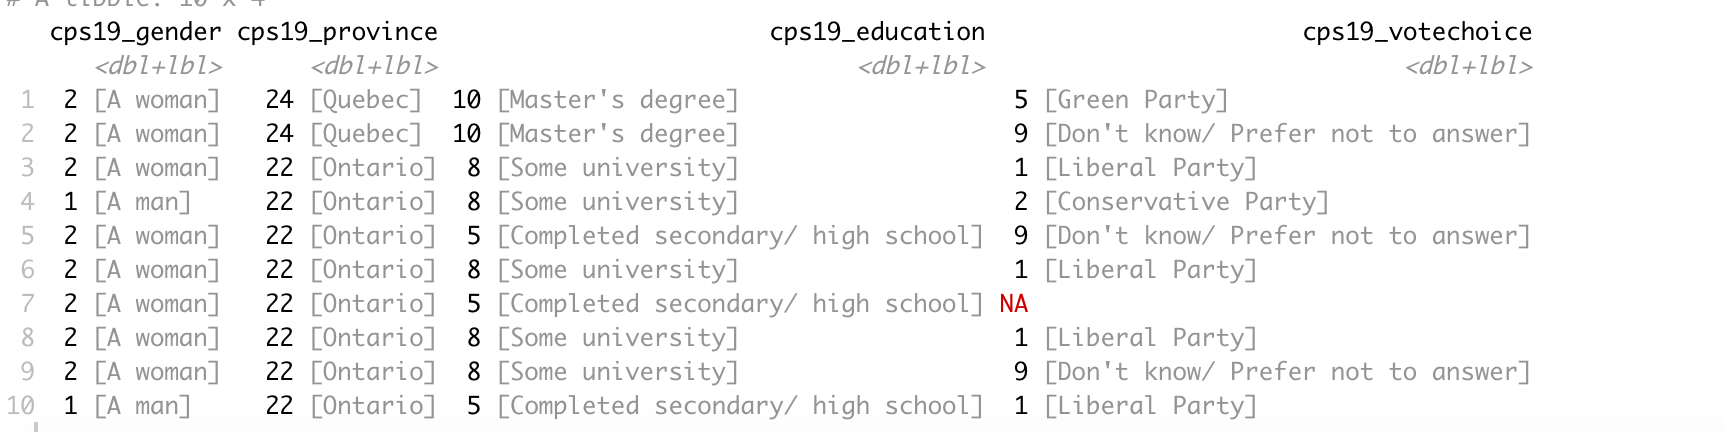
\includegraphics[height=4in]{P1.png}
    \caption{Description of Vote data}
\end{figure}

\hypertarget{result}{%
\subsection{Result}\label{result}}

Based on the result of models, we may conclude several interesting
things. First, the intercept for male is negative while the intercept
for female is positive, it would imply that male tend to vote for
Liberal party while female tend to vote for Conservative Party. We also
noticed that the willingness to vote for Conservative Party tends to
decline as people has higher educational level. It implies that people
with higher education tend to vote for Conservative Party and people
with lower education tend to vote for Liberal Party.

\begin{figure}
    \centering
    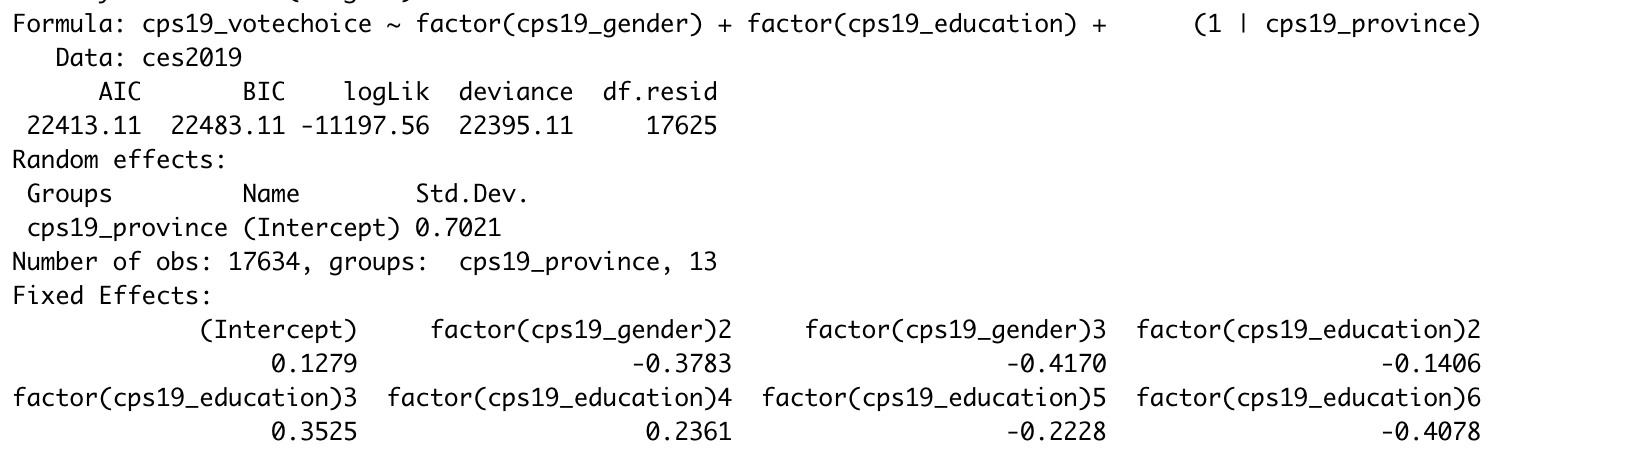
\includegraphics[height=4in]{P2.png}
    \caption{Model Interpretation}
\end{figure}

For generalized linear model, the posterior probability that
Conservative Party wins is 0.462, versus the wining probability equals
to 0.538 for Liberal Party. For linear model, the posterior probability
that Conservative Party wins is 0.461, versus the wining probability
equals to 0.539 for Liberal Party. We may see that both models have
similar posterior probability, and both of the results imply that
Liberal Party has a little higher wining probability than Conservative
Party. We are likely to say Liberal Party is more likely to win the
election in 2020 because of the higher posterior probability

\hypertarget{discussion}{%
\subsection{Discussion}\label{discussion}}

In summary, we successfully building an MRP model based on CES and
post-hierarchical data sets to predict who will get more popular votes
in the Canadian federal election in 2019 by using the survey data set
2019 CES online survey to observe the demographic data.

Based on out data analysis, we draw an conclusion that the winning
probabilities for Liberal Party is a little higher than Conservative
Party. Our secondary outcome is that female tend to vote for
Conservative Party and male tend to vote for Liberal party. High
educated people also tend to vote for Liberal Party.

In general, our method provides some broader methodological guidance for
dealing with voting surveys. In our model, we simply the variable to
gender, education level and state. In practice, the appropriateness of
the model depends on the variables used, the relationship between those
variables and the opinion being modeled, and the relationship between
unmeasured variables and the opinion being modeled. One author
improvement could involve more variables in the model and explore which
variable could be useful in prediction.

Another possible improvement would be about the model itself, we build a
logistic model with binary outcome. Researchers could also build
multi-level outcome models to improve the prediction accuracy. We could
also consider relationships of our variable, for example, to detect
interaction between two models.

\hypertarget{reference}{%
\subsection{Reference}\label{reference}}

1.Government of Canada, S. (2017, November 27). Education Highlight
Tables, 2016 Census. Retrieved December 09, 2020, from
\url{https://www12.statcan.gc.ca/census-recensement/2016/dp-pd/hlt-fst/edu-sco/index-eng.cfm}

2.The Canadian Election Study Dataset.
\url{https://hodgettsp.github.io/cesR/}

3.Bailey, Michael A., Daniel J. Hopkins \& Todd Rogers, 2016,
`Unresponsive and Unpersuaded: The Unintended Consequences of a Voter
Persuasion Effort', Political Behavior

4.MRP with rstanarm,
\url{https://cran.r-project.org/web/packages/rstanarm/vignettes/mrp.html}

\end{document}
